\documentclass[12pt]{article}
\usepackage[utf8]{inputenc}
\usepackage[T1]{fontenc}
\usepackage[polish,provide=*]{babel}
\usepackage{amsmath,amssymb,amsfonts}
\usepackage{latexsym}
\usepackage{siunitx}
\sisetup{
  locale = DE,
  separate-uncertainty = true,
  per-mode = symbol
}
\usepackage{graphicx}
\usepackage{subcaption}
\usepackage{float}
\graphicspath{{./images/}}
\usepackage{booktabs}
\usepackage{enumitem}
\usepackage{hyperref}
\hypersetup{colorlinks=true, linkcolor=blue, citecolor=blue, urlcolor=blue}

\setlength{\parindent}{0pt}
\setlength{\oddsidemargin}{0in}
\setlength{\textwidth}{6.5in}
\setlength{\textheight}{8.8in}
\setlength{\topmargin}{0in}
\setlength{\headheight}{18pt}

\title{Przemiany gazowe}
\author{Kacper Kłos}
\date{\today}

\begin{document}

\maketitle

W niniejszym raporcie analizujemy zachowanie powietrza podczas dwóch przemian gazowych. 
Najpierw przeprowadziliśmy \textbf{przemianę izochoryczną} w celu wyznaczenia temperatury zera bezwzględnego \(T_0\) oraz liczby moli \(n\) zamkniętego gazu. Z dwóch serii pomiarowych otrzymaliśmy
\begin{align*}
  T_{0,1} &= \SI{-287\pm 8}{\celsius}, & n_1 &= \SI{20.1\pm0.7e-3}{\mole},\\
  T_{0,2} &= \SI{-282\pm 6}{\celsius}, & n_2 &= \SI{20.2\pm0.5e-3}{\mole},
\end{align*}
co po uśrednieniu ważonym daje \(T_0 = \SI{-284\pm 5}{\celsius}.\)

Następnie wykonaliśmy \textbf{przemianę izotermiczną}, badając zakres stosowalności równania gazu doskonałego oraz ponownie wyznaczając \(n\). Otrzymano zakresy ciśnień
\begin{align*}
  P_1 &\in \left[\SI{105.5}{\kilo\pascal};\,\SI{152.1}{\kilo\pascal}\right], &
  n_1 &= \SI{4.4\pm0.7e-3}{\mole},\\
  P_2 &\in \left[\SI{55.6}{\kilo\pascal};\,\SI{63.9}{\kilo\pascal}\right], &
  n_2 &= \SI{2.30\pm0.17e-3}{\mole}
\end{align*}
Także wyznaczyliśmy jaka objętość powietrza znajduje się w układzie poza kontrolowaną przez nas strzykawką
\[
    V_{0,1} = \SI{45.7\pm1.3}{\milli\liter}, \quad V_{0,2} = \SI{45.1\pm6.8}{\milli\liter} 
\]
O średniej ważonej \(V_0 = \SI{45.7\pm1.3}{\milli\liter}\).

\newpage
\section{Aparatura pomiarowa i przyjęte stałe}
\begin{itemize}[leftmargin=*]
  \item \textbf{Czujnik ciśnienia} PASCO PS-3203\cite{pressure} (dokładność: \SI{\pm2}{\kilo\pascal}).
  \item \textbf{Czujnik temperatury} PASCO PS-3222\cite{temperature} (dokładność: \SI{\pm0.5}{\celsius}).
  \item \textbf{Stała gazowa}: \(R = \SI{8.314}{\joule\per\mole\per\kelvin}\)\cite{gas_const}.
  \item \textbf{Temperatura zera bezwzględnego}: \(T_0 = \SI{-213.15}{\celsius}\)\cite{zero}.
\end{itemize}

\section{Przemiana izochoryczna}
Gaz zamknięto w miedzianej kuli o promieniu \SI{2}{in} (\SI{1}{in} = \SI{2.54}{cm}). Wnętrze wyposażono w wymienione wyżej czujniki. Kulę zanurzono w wodzie w izolowanym pojemniku i ogrzewano strumieniem wrzątku. W momencie osiągnięcia równowagi termodynamicznej zapisywano pomiary czujników i procedure powtarzano.

\begin{table}[H]
  \centering
  \begin{tabular}{c|cc|cc}
    \toprule
    \textbf{Nr} & $T_1$ [\si{\celsius}] & $P_1$ [\si{\kilo\pascal}] & $T_2$ [\si{\celsius}] & $P_2$ [\si{\kilo\pascal}] \\
    \midrule
    1  &  5,9 &  95,1 &  7,9 &  87,6 \\
    2  & 12,7 &  97,4 & 18,0 &  91,2 \\
    3  & 17,2 &  98,9 & 27,0 &  94,1 \\
    4  & 23,6 & 100,6 & 31,2 &  95,6 \\
    5  & 29,6 & 102,7 & 37,1 &  98,3 \\
    6  & 34,7 & 104,9 & 40,7 &  99,1 \\
    7  & 40,1 & 106,5 & 47,5 & 100,7 \\
    8  & 46,3 & 108,1 & 50,3 & 101,4 \\
    9  & 52,3 & 108,9 & 53,9 & 102,6 \\
    10 & 58,5 & 110,6 & 57,5 & 103,8 \\
    11 & 64,0 & 113,8 & 60,9 & 104,6 \\
    12 & 71,1 & 114,9 & 65,6 & 105,8 \\
    13 & 79,4 & 119,4 & 70,0 & 106,9 \\
    14 & 84,8 & 122,1 & 75,4 & 109,3 \\
    15 &  --  &   --  & 81,6 & 110,2 \\
    \bottomrule
  \end{tabular}
  \caption{Wyniki pomiarów dwóch serii badania przemiany izochorycznej: temperatura \(T\) (niepewność \SI{0.5}{\celsius}) oraz ciśnienie gazu \(P\) (niepewność \SI{2}{\kilo\pascal}).}
  \label{tab:isochoric_measurements}
\end{table}

Przyjmując, że w badanym zakresie powietrze zachowuje się jak gaz doskonały, opisuje je równanie
\[
  PV = nR\left(T - T_0\right)
\]
Ze względu na to, że błąd pomiaru temperatury jest znacznie mniejszy od błędu pomiaru ciśnienia (od \SI{2}{\%} do \SI{0.2}{\%} w badanym zakresie), regresję liniową prowadzimy z \(T\) jako zmienną niezależną.
\[
  P = aT + b, \quad a = \frac{nR}{V}, \; b = -\frac{nRT_0}{V}
\]
\begin{figure}[H]
  \centering
  \begin{subfigure}{0.47\textwidth}
    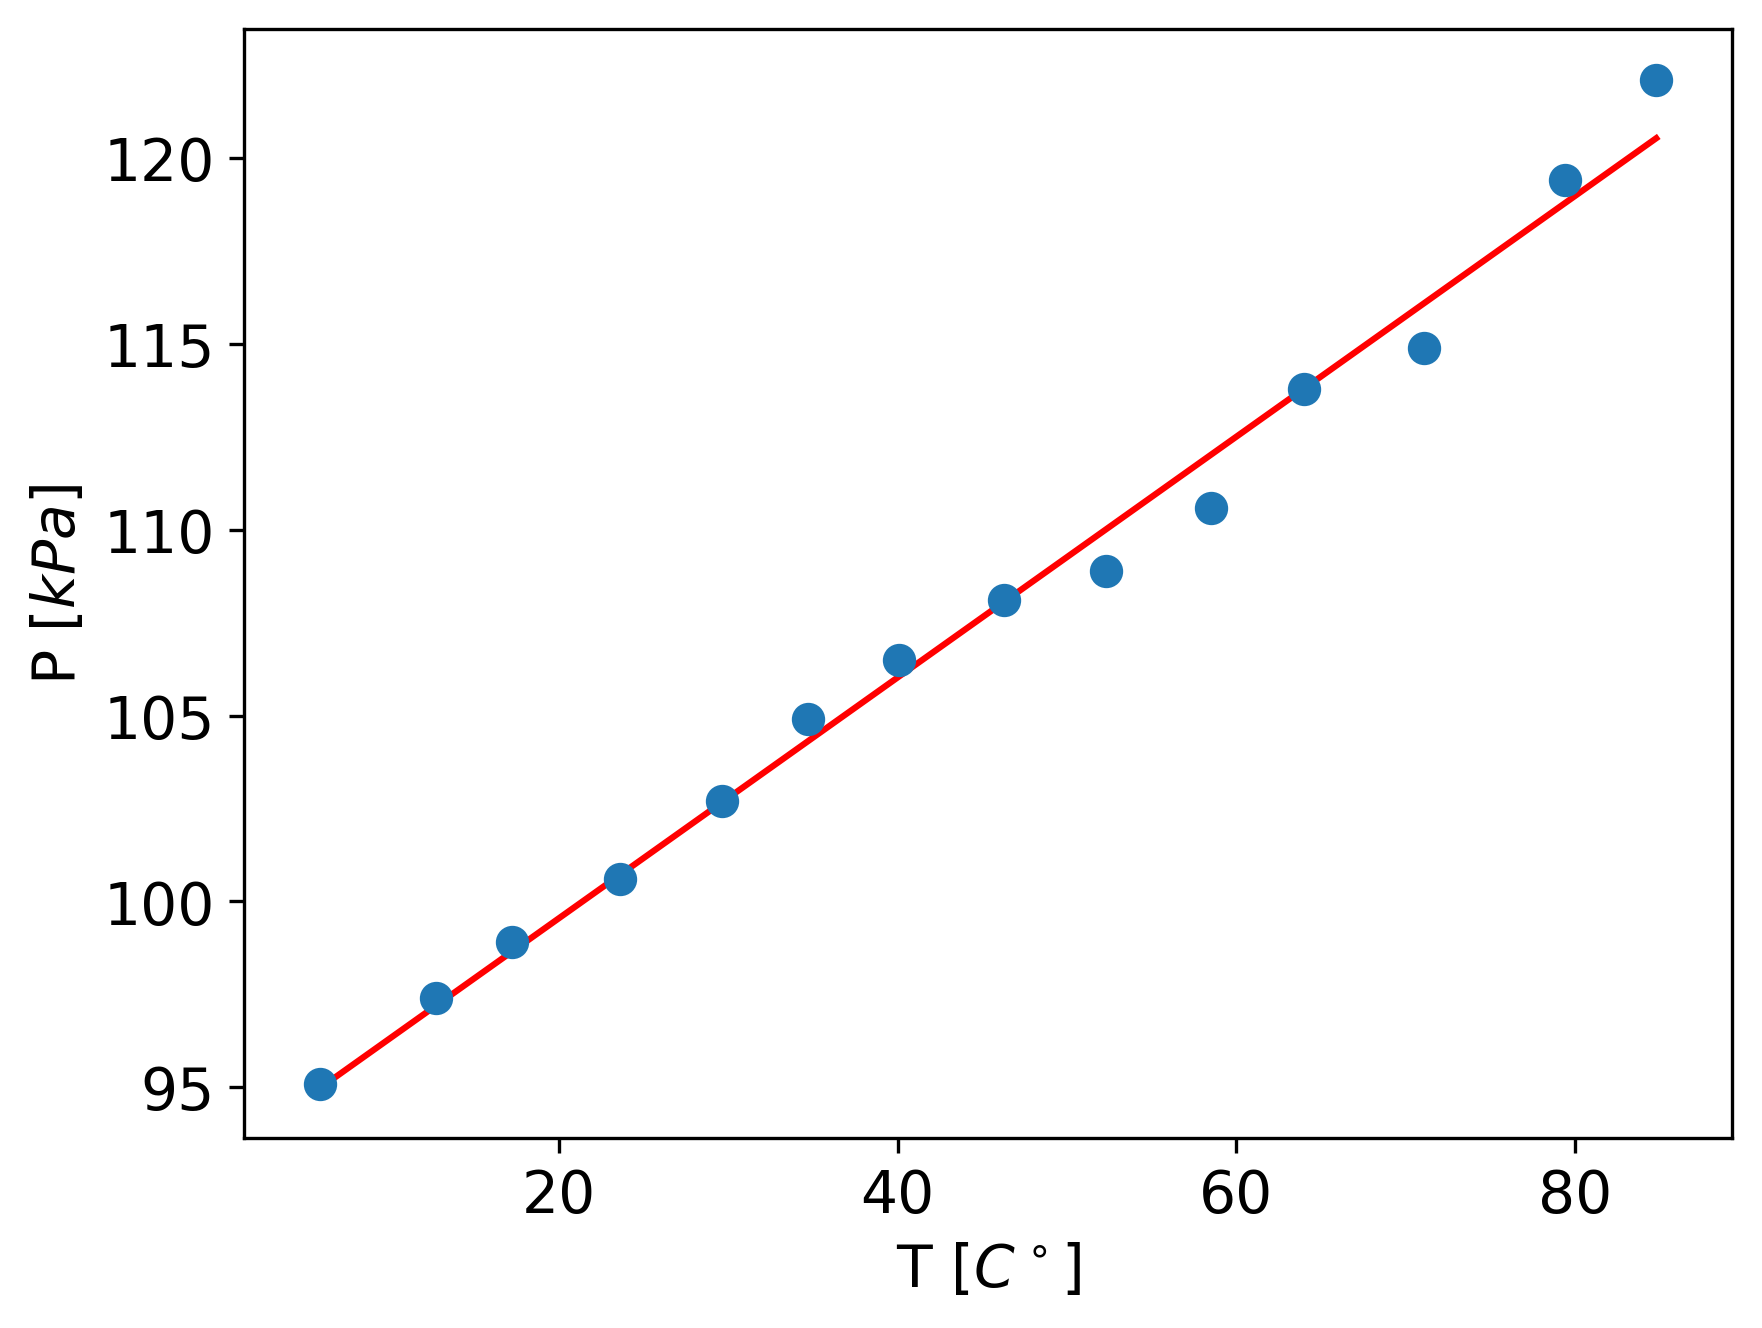
\includegraphics[width=\linewidth]{izohoric_0}
    \caption{Seria 1}
  \end{subfigure}\hfill
  \begin{subfigure}{0.47\textwidth}
    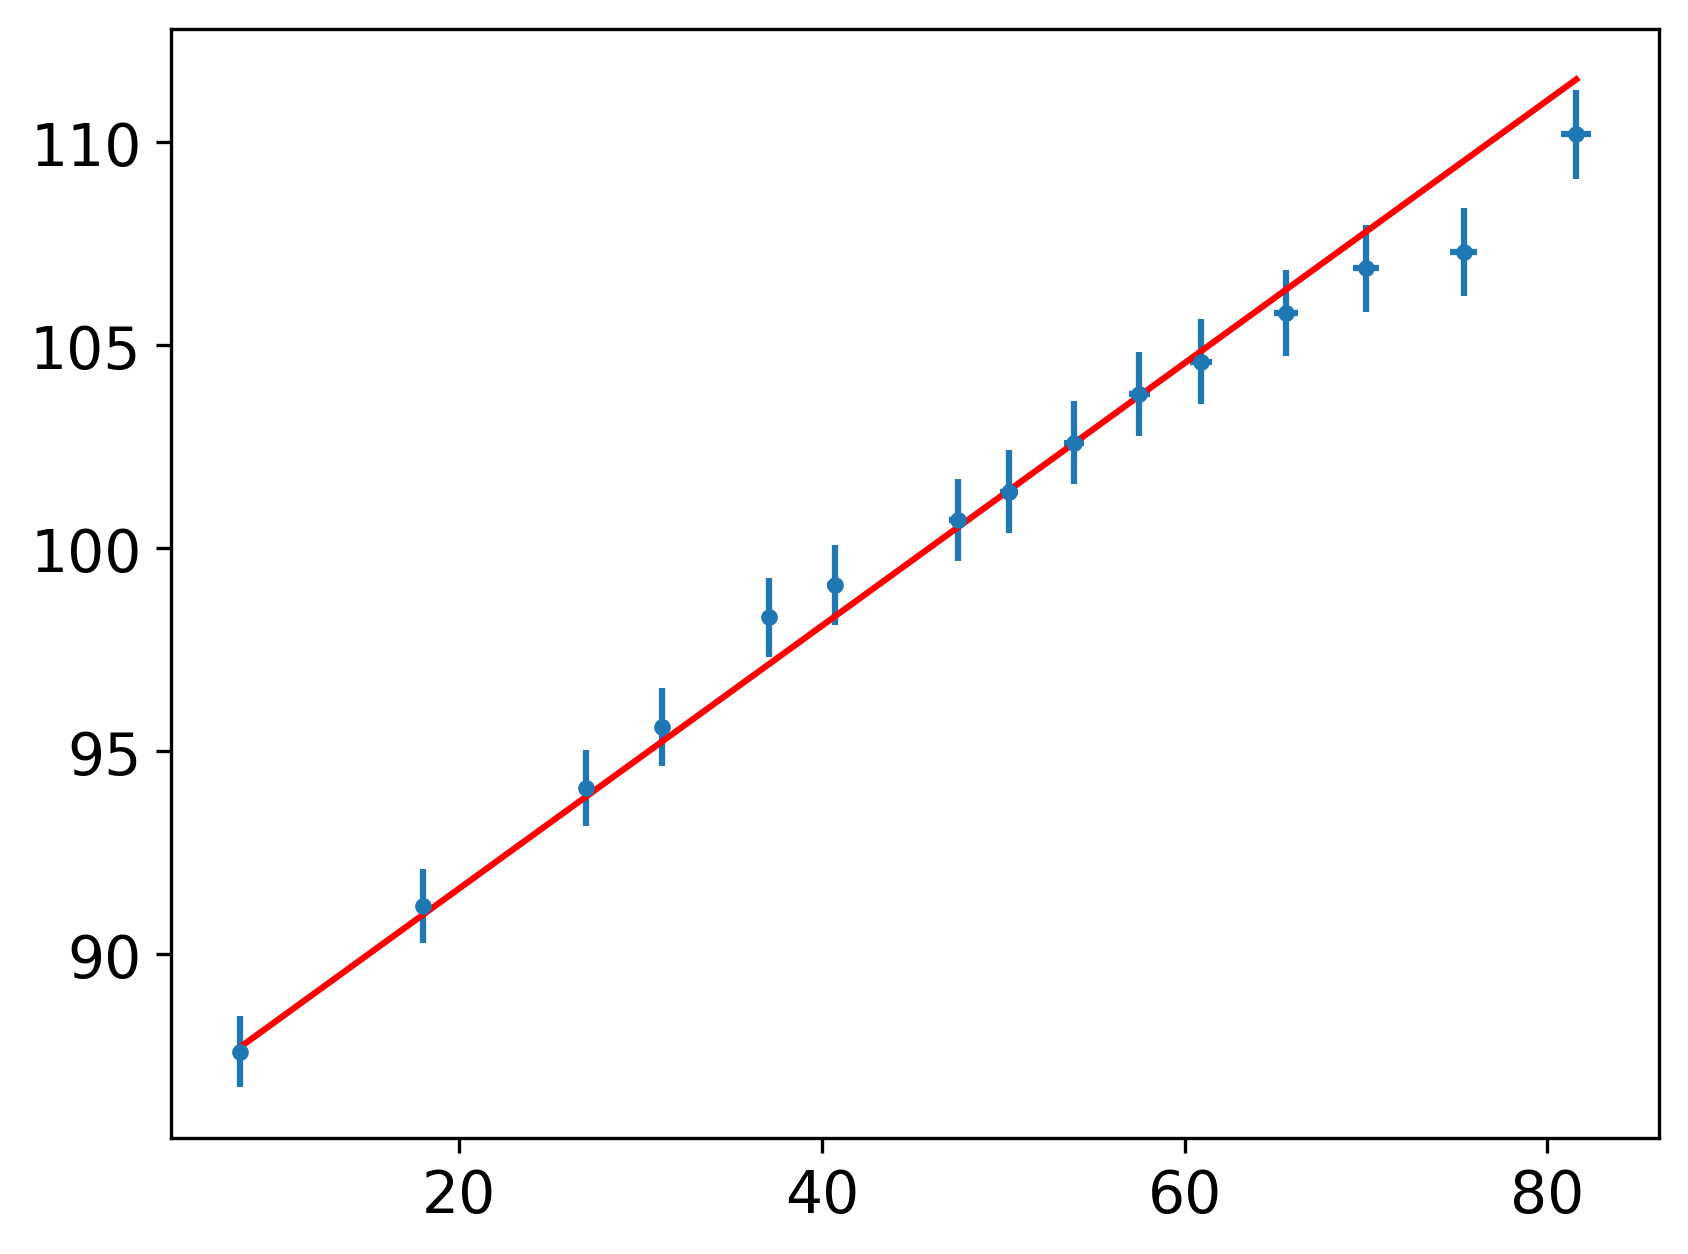
\includegraphics[width=\linewidth]{izohoric_1}
    \caption{Seria 2}
  \end{subfigure}
  \caption{Zależność ciśnienia \(P\) od temperatury \(T\) dla gazu o stałej objętości. Czerwone linie przedstawiają dopasowanie liniowe.}
  \label{fig:izohoric}
\end{figure}
Dopasowanie daje współczynniki
\begin{align*}
  a_1 &= \SI{0.320\pm0.010}{\kilo\pascal\per\celsius}, & b_1 &= \SI{93.1\pm0.5}{\kilo\pascal}\\
  a_2 &= \SI{0.305\pm0.006}{\kilo\pascal\per\celsius}, & b_2 &= \SI{86.0\pm0.3}{\kilo\pascal}
\end{align*}
Z nich wyznaczamy
\[
  T_0 = -\frac{b}{a}, \qquad n = \frac{aV}{R}
\]
co przy objętości kuli \(V = \frac{4}{3}\pi r^3 = \SI{5.49e-4}{\meter^3}\) (\(r = \SI{2}{in} = \SI{5.08}{cm}\)) prowadzi do wyników.
\begin{align*}
  T_{0,1} &= \SI{-287\pm 8}{\celsius}, & n_1 &= \SI{20.1\pm0.7e-3}{\mole}\\
  T_{0,2} &= \SI{-282\pm 6}{\celsius}, & n_2 &= \SI{20.2\pm0.5e-3}{\mole}
\end{align*}
co po uśrednieniu ważonym daje \(T_0 = \SI{-284\pm 5}{\celsius}\).

\newpage 

\section{Przemiana izotermiczna}
Gaz został zamknięty w strzykawce której koniec połączono przewodami z czujnikami. Po przestawieniu tłoka czekaliśmy, aż temperatura powróci do wartości otoczenia \(T = \SI{23.0\pm0.1}{\celsius}\) rejestrując ciśnienie i objętość wskazywaną przez strzykawkę.

\begin{table}[H]
  \centering
  \begin{tabular}{c|cc|cc}
    \toprule
    \textbf{Nr} & $V_1$ [\si{\milli\liter}] & $P_1$ [\si{\kilo\pascal}] & $V_2$ [\si{\milli\liter}] & $P_2$ [\si{\kilo\pascal}] \\
    \midrule
    1  & 60 &  99,6 & 26 & 99,6 \\
    2  & 56 & 105,5 & 30 & 87,4 \\
    3  & 52 & 110,4 & 34 & 78,8 \\
    4  & 48 & 116,0 & 38 & 73,1 \\
    5  & 44 & 121,1 & 42 & 68,0 \\
    6  & 41 & 125,3 & 46 & 63,9 \\
    7  & 37 & 130,5 & 50 & 60,7 \\
    8  & 33 & 137,7 & 54 & 57,9 \\
    9  & 29 & 144,8 & 58 & 56,3 \\
    10 & 26 & 152,1 & 60 & 55,6 \\
    \bottomrule
  \end{tabular}
  \caption{Dane pomiarowe dla dwóch serii przemiany izotermicznej: objęctość wskazywana przez strzykawkę \(V\) (niepewność \(\SI{1.2}{\milli\liter}\)) oraz ciśnienie P (niepewność \(\SI{2}{\kilo\pascal}\)).}
  \label{tab:isothermal_data}
\end{table}

Teoretycznie powinno zachodzić równanie
\[
  \frac{P\,(V+V_0)}{T - T_0} = nR = \text{const}
\]
W którym $V_0$ oznacza objętość gazu zawartego w przewodach.
Równanie można zapisać w postaci liniowej
\[
  \frac{PV}{T - T_0} = aP + b, \quad a = -\frac{V_0}{T - T_0}, \; b = nR
\]
Stosując profesjonalnie wyznaczoną temperature zera bezwzględnego \(T_0 = \SI{-213.15}{\celsius}\) dopasowujemy stałe $a$ i $b$ tak żeby jak najtrafniej opisywały nasze dane w zakresie liniowym.
\begin{figure}[H]
  \centering
  \begin{subfigure}{0.47\textwidth}
    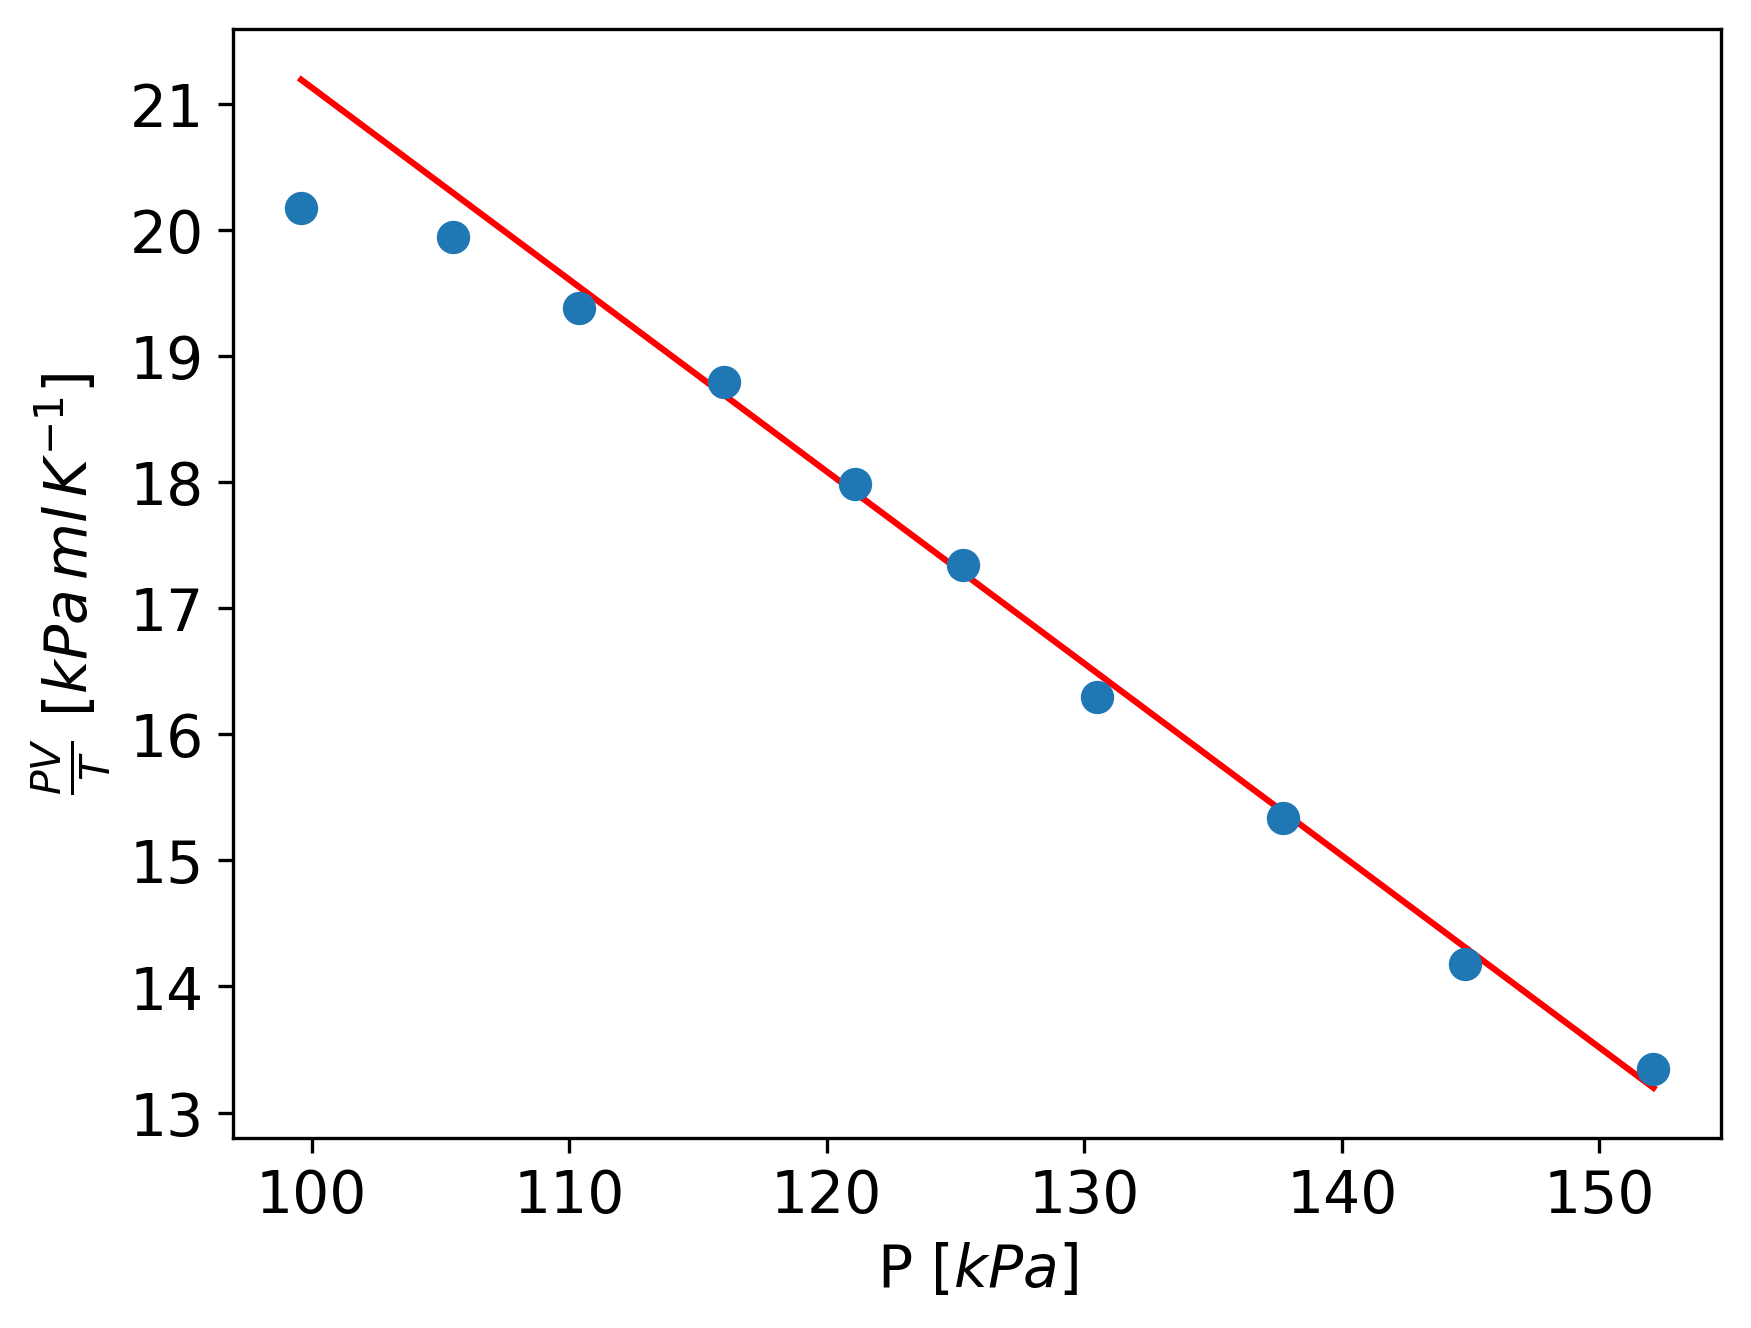
\includegraphics[width=\linewidth]{izotermic_0}
    \caption{Seria 1 — sprężanie}
  \end{subfigure}\hfill
  \begin{subfigure}{0.47\textwidth}
    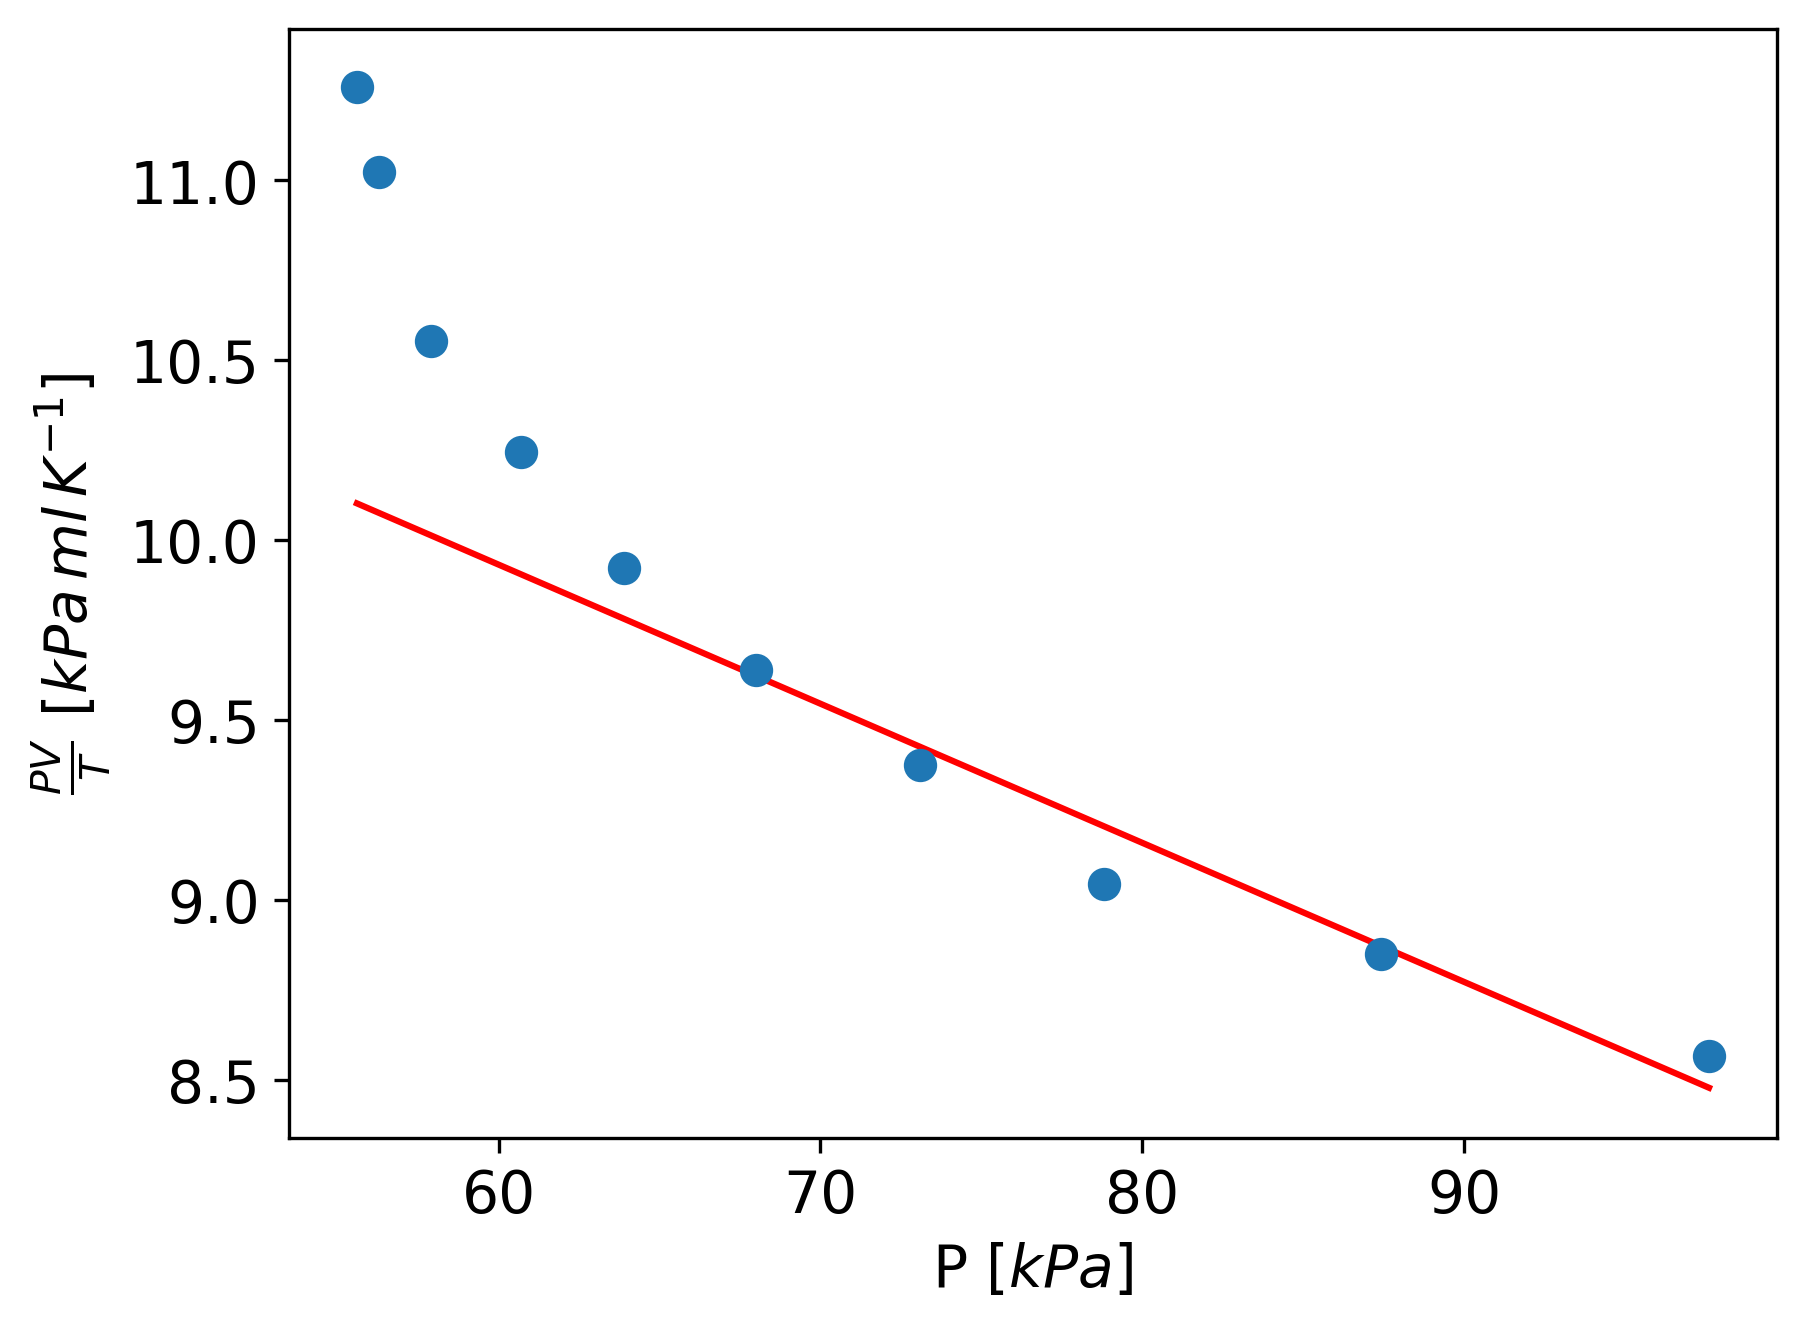
\includegraphics[width=\linewidth]{izotermic_1}
    \caption{Seria 2 — rozprężanie}
  \end{subfigure}
  \caption{Zależność $\tfrac{PV}{T - T_0}$ od ciśnienia $P$ przy $T = \SI{23.0\pm0.1}{\celsius}$. Czerwone linie to dopasowanie liniowe w zakresie stosowalności równania gazu doskonałego.}
  \label{fig:isothermal}
\end{figure}
Widzimy że zakres w którym niepewność punktów pomiarowych nie osiągają dopasowanej prostej wynosi 
\[
  P_1 \in \left[\SI{105.5}{\kilo\pascal};\,\SI{152.1}{\kilo\pascal}\right], \quad
  P_2 \in \left[\SI{55.6}{\kilo\pascal};\,\SI{63.9}{\kilo\pascal}\right]
\]
Ten zakres uznajemy za przedział aplikowalności równania gazu doskonałego.


Dopasowane krzywe liniowe odpowiadają parametrą
\begin{align*}
  a_1 &= \SI{-0.154\pm0.005}{\milli\liter\kelvin^{-1}}, & b_1 &= \SI{36.6\pm0.6}{\pascal\liter\kelvin^{-1}}\\
  a_2 &= \SI{-0.152\pm0.023}{\milli\liter\kelvin^{-1}}, & b_2 &= \SI{19.6\pm1.4}{\pascal\liter\kelvin^{-1}}
\end{align*}
Liczbę moli wyznaczamy z relacji
\[
  n = \frac{b}{R}
\]
Otrzymujemy w ten sposób wyniki
\[
  n_1 = \SI{4.4\pm0.7e-3}{\mole}, \quad n_2 = \SI{2.3\pm0.17e-3}{\mole}.
\]
Możemy również oszacować zawartość gazu w przewodach
\[
    V_0 = -a (T-T_0)
\]
Z czego wynika
\[
    V_{0,1} = \SI{45.7\pm1.3}{\milli\liter}, \quad V_{0,2} = \SI{45.1\pm6.8}{\milli\liter} 
\]
O średniej ważonej
\[
    V_0 = \SI{45.7\pm1.3}{\milli\liter}
\]

\newpage

\section{Podsumowanie}
Otrzymana wartość temperatury zera bezwzględnego \(T_0 = \SI{-284\pm5}{\celsius}\) jest dość dokładna, świadczy o tym fakt że zawiera w swoim przedziale \(3\sigma\) wartość wyznaczoną profesjonalnie\cite{zero} \(T_0 = \SI{-273.15}{\celsius}\). 

Głównym źródłem niepewności w części izochorycznej był błąd pomiarowy ciśnienia, będący znacznie większy od błędu mierzonej temperatury. Trzeba wspomnieć o tym że trudność sprawiało stwierdzenie w którym momencie układ osiągnął równowagę cieplną, szczególnie w przypadku wysokich temperatur dla których temperatura zauważalnie maleje z czasem, co również wprowadza trudny do określenia błąd.

Dla przemiany izotermicznej zauważamy że liczba moli wpływa istotnie na zakres ciśnień, dla którego powietrze można traktować jako gaz doskonały. Dla większego \(n\) uzyskano zakres wyższych ciśnień, natomiast przy mniejszej \(n\) zakres przesunął się do niższych ciśnień, a charakter odchylenia od prostoliniowości zmienił znak krzywizny.
Jednak trudno stwierdzić czy wskazane liczby w drugiej serii są poprawne gdyż wymagające było wybranie zakresu liniowego. Uzyskane przez nas dane były widocznie nie liniowe, podczas dopasowywania prostej mogliśmy równie dobrze uznać że liniowo zachowuje się zakres dla zakresu wysokich ciśnień. Wybraliśmy jednak taki zakres który zapewniał lepszą zgodność z objętością wyznaczoną w serii pierwszej, którą bardzo dobrze opisywała zależność liniowa.

W pomiarach izotermicznych również dominował błąd wynikający z pomiaru ciśnienia. Znaczący wpływ miała nieidealna szczelności układu, po zmianie objętości obserwowano stopniowy dryf ciśnienia ku wartościom atmosferycznym, efekt mógł się kumulować wraz z pomiarami mając największy wpływ na te wykonane na końcu serii.

\vspace{1 in}

\begin{thebibliography}{5}
  \bibitem{temperature} Czujnik temperatury PASCO PS-3222 \url{https://cdn.pasco.com/product_document/Wireless-Temperature-Link-Manual-PS-3222_1_.pdf}
  \bibitem{pressure}   Czujnik ciśnienia PASCO PS-3203 \url{https://www.pasco.com/products/sensors/wireless/wireless-pressure-sensor#documents-panel}
  \bibitem{skrypt}      A. Drabińska, \emph{Badanie przemian gazowych. Wyznaczanie temperatury zera bezwzględnego}, Uniwersytet Warszawski.
  \bibitem{gas_const}   Stała gazowa \url{https://physics.nist.gov/cgi-bin/cuu/Value?r}
  \bibitem{zero}        Temperatura zera bezwzględnego \url{https://www.bipm.org/documents/20126/41483022/SI-Brochure-9-EN.pdf/2d2b50bf-f2b4-9661-f402-5f9d66e4b507}
\end{thebibliography}

\end{document}
